\chapter{绪论:初识机器学习}

\begin{center}
学而不思则罔,思而不学则怠!
\end{center}

\begin{flushright}
---孔子    
\end{flushright}

\section{欢迎参加机器学习课程}

写 ElegantNote 模板的初衷是为了简化我在写笔记中的工作,因为我不会写类文件和包文件,所以,最当初是想拜托小L做出一个华丽,
清爽的 \LaTeX{} 模板,最好是类文件,而且因为这样可以简化导言区复杂的内容。后来,和小L一拍即合,遂开始一起做Elegant\LaTeX{}的设计。

在学校的时候,搞定了定理环境样式的代码。因为不想重复 China\TeX{} 那个经典的页眉页脚,我找到了计量书上的一个图案,小L拿 Ti\emph{k}Z 一点一点把那个画出来了,不过我最后还是用的截取的方式得到的图案。慢慢地,我们把初步的样子做出来了。

2013年的暑假开始后,我对那个初步的模板做了一点改动,然后用它写了Dynamic Programing 的笔记,并且,在写的过程中,对模板加了封面,也就是模板现在的封面(logo 在Version 2.00中已经改了)。至此,模板的大致样子终于出来了,不过当时也在写笔记的过程中知道了某些不足,比如
\begin{enumerate}
\item 定理类的环境在我们这个模板中不能浮动,也不能跨页,在Version 2.00 版本中已经添加。
\item 某些环境不足,比如例子、假设、性质、结论等环境,在1.00版本中已经增加了这几个环境,在2.00版本中,环境设置更加全面。
\item 一些我们不可预知的错误将会不期而遇。
\item 一些我们目前没有需求,但是可以继续改进的地方,比如表格样式,比如抄录样式等。
\end{enumerate}

写完那个笔记之后越发让我对 Elegant\LaTeX{} 模板的制作更有激情,在和小L相互讨论的几天里,我们终于得到了1.00 版本的 ElegantNote 模板。

\section{什么是机器学习?}

在实际应用中,我们发现了一个比较重要的问题,因为在一般的笔记中,定义、定理经常一起出现,和课本区别比较大的是,通常是一堆定义之后,出现一堆性质或者定理。如果出现这种情况,使用 ElegantNote 模板会导致分块很严重,影响排版质量和美观。思前想后,我们决定将 ElegantNote 模板更新为 ElegantBook 模板,并在未来重新设计一个简洁版本的 ElegantNote。 至此ElegantBook 才横空出世,由于更名原因,ElegantBook 1.00 版本也即原来的 ElegantNote, 而ElegantBook 2.00 为目前的正式版本。

\section{监督学习}

我以前从未写过类文件,所以,写这个模板的过程必然是折腾的过程,在写模板的过程中,最主要参考了《写给\LaTeXe{} 类与宏包的作者》\cite{packagewriter}、moderncv.cls 文件、\href{http://aff.whu.edu.cn/huangzh/}{武汉大学黄正华老师的论文模板}、《\LaTeXe{} 完全学习手册》\cite{complete}、{\itshape The Not So Short Introduction to \LaTeXe{}}\cite{oetiker2010not}以及各大\LaTeX{} 疑问解答网站,在此为无私奉献的组织和个人表示感谢!

{\color{thid}忍不住插个图!}

\begin{figure}[!hbtp]
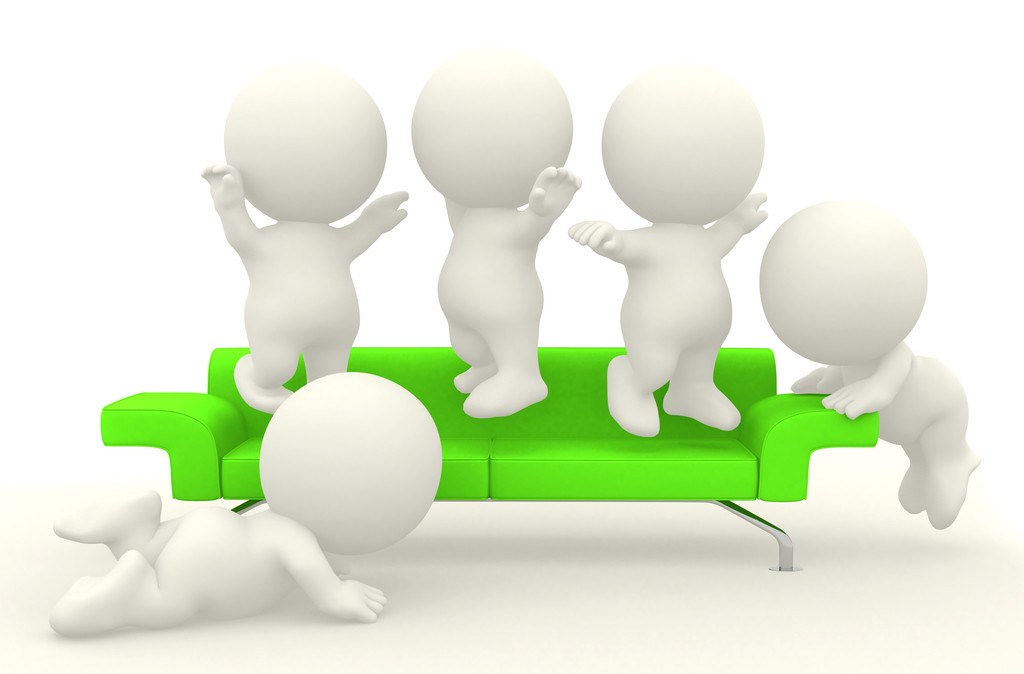
\includegraphics[width=0.8\textwidth]{happy.jpg}
\caption{Happiness,we have it!\label{figur:happy}}
\end{figure}

\section{无监督学习}

\section{问题}